\documentclass[11pt]{article}

\usepackage{setspace}
\usepackage{amsmath}
\usepackage{enumitem}
\usepackage{amsfonts} 
\usepackage{mathtools}
\usepackage{relsize}
\usepackage{graphicx}
\usepackage[top=2cm,bottom=2cm,left=2.5cm,right=2.5cm,marginparwidth=1.75cm]{geometry}
\setlength{\parindent}{0cm}
\usepackage{listings}
\usepackage{clrscode3e}
\usepackage{graphicx}

\title{\vspace{-1.0cm}PHYS 2303 Homework 6}
\author{Fletcher Gornick}
\date{February 26, 2022}

\spacing{1.5}
\begin{document}
 \maketitle
 \section*{Chapter 1 Problem 60}
 A narrow beam of light containing red (660 nm) and blue (470 nm) wavelengths travels from air 
 through a 1.00-cm-thick flat piece of crown glass and back to air again. The beam strikes at a 
 \(30.0^\circ\) incident angle. \\\\
 (a) At what angles do the two colors emerge? \\\\
 (b) By what distance are the red and blue separated when they emerge?
 \newpage

 \section*{Chapter 1 Problem 92}
 A light ray entering an optical fiber surrounded by air is first refracted and then reflected 
 as shown below. Show that if the fiber is made from crown glass, any incident ray will be totally 
 internally reflected. \\\\
 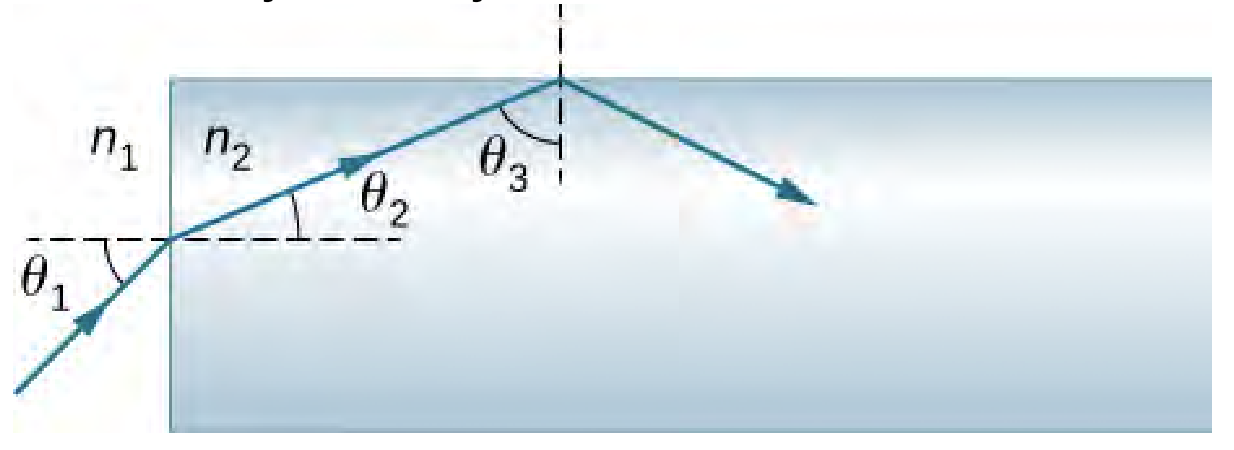
\includegraphics[scale=0.5]{1-92.png}
 \newpage

 \section*{Chapter 1 Problem 93}
 A light ray falls on the left face of a prism (see below) at the angle of incidence \(\theta\) 
 for which the emerging beam has an angle of refraction \(\theta\) at the right face. Show that 
 the index of refraction \(n\) of the glass prism is given by
 \[n = \displaystyle\frac{\sin \frac12 (\alpha + \phi)}{\sin \frac12 \phi}\]
 where \(\phi\) is the vertex angle of the prism and \(\alpha\) is the angle through which the 
 beam has been deviated. If \(\alpha = 37.0^\circ\) and the base angles of the prism are each 
 \(50.0^\circ\), what is \(n\)? \\\\
 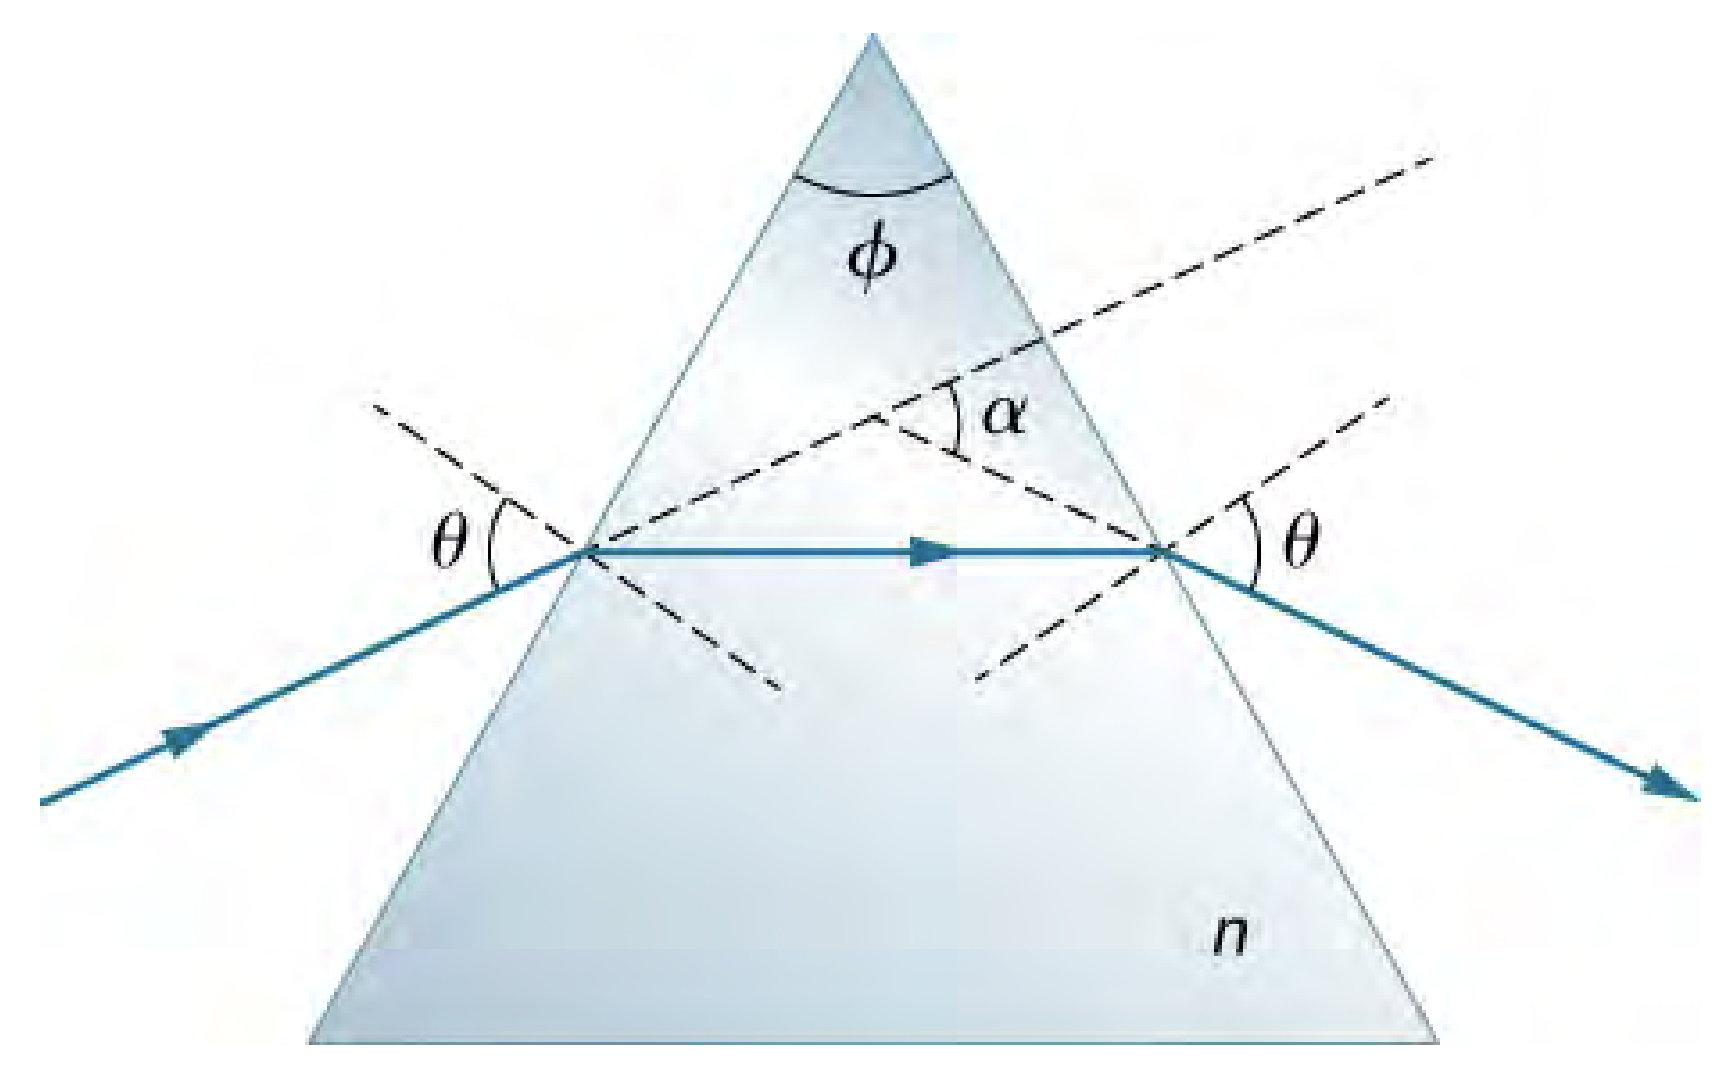
\includegraphics[scale=0.3]{1-93.png}
 \newpage

 \section*{Chapter 2 Problem 36}
 A shopper standing 3.00 m from a convex security mirror sees his image with a magnification of 
 0.250. \\\\
 (a) Where is his image? \\\\
 (b) What is the focal length of the mirror? \\\\
 (c) What is its radius of curvature? \\\\
\end{document}
